\subsection{Challenges, Limitations, and Future Avenues}

There are important challenges and limitations to ARC-task generation in general, as well as limitations specific to our particular algorithm.  

\subsubsection{Assessing Task Validity}

The original ARC tasks were entirely generated and verified by humans. The fact that often several humans verified and successfully solved them showcases their validity. However, when algorithmically generating tasks, since we to date have no satisfactory solver to generate tasks, there is no way to confidently assess the validity of the generated task. Specifically, there are two category of problems one may run into when generating tasks, for which there is no easy algorithmic fix.

\begin{itemize}
    \item \textbf{Overdetermined tasks:} Given the training examples, there exists more than one unique strategy to solve the task. While this often is not a critical issue, it can happen that some of the rules lead to different solutions in the test example, thereby leading to an error originating from the ambiguity of the task rather than the solver. 
    \begin{figure}[H] 
    \centering
    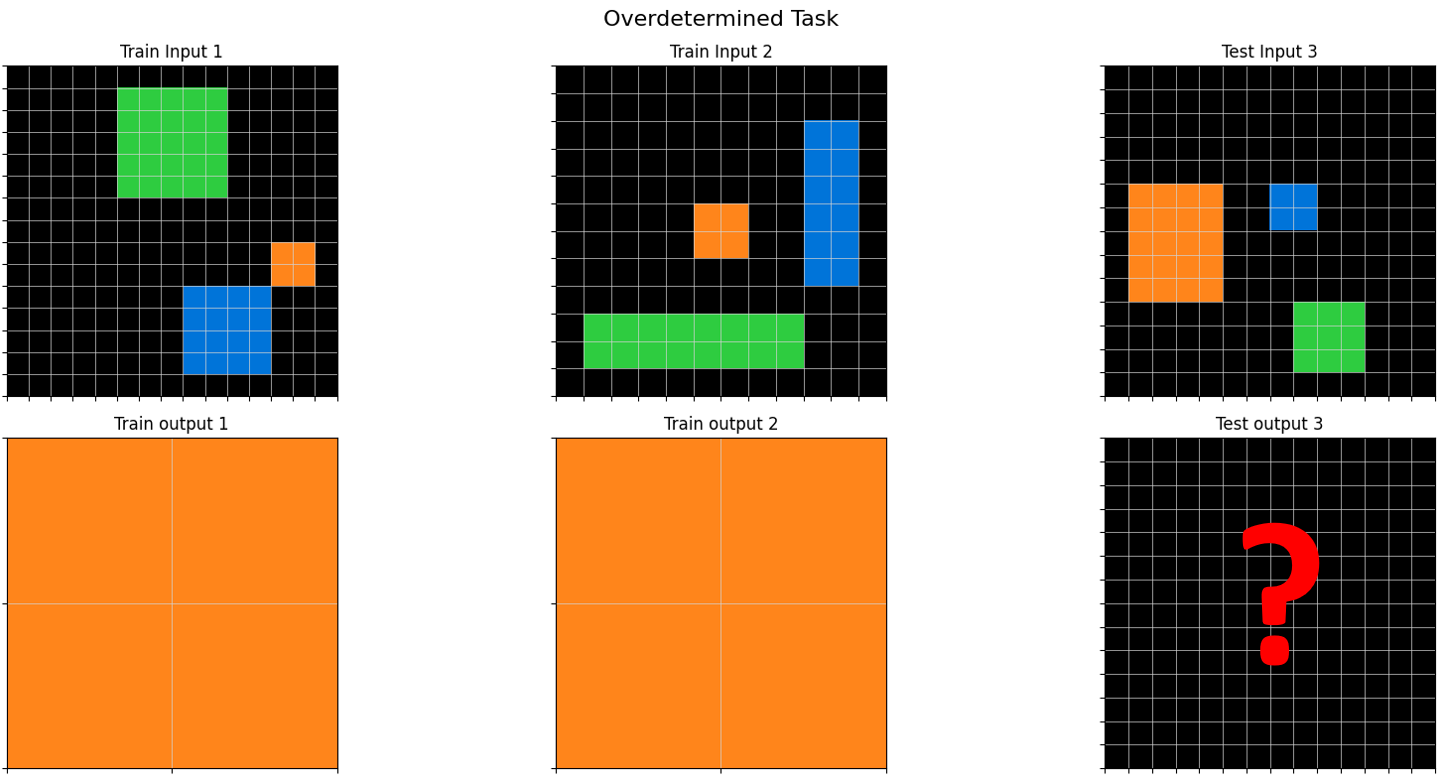
\includegraphics[width=0.6\columnwidth]{Figures/Overdetermined_Task.png}
    \caption{Overdetermined task. It is impossible to infer from the two training examples whether the rule is "Select orange object" or "Select smallest object", as both rules are valid in the two training examples. We therefore cannot solve the test example.}
    \label{fig:Overdetermined Task}
\end{figure}
    \item \textbf{Underdetermined tasks:} Given the training examples, we cannot find a single rule that works for all cases presented. This makes the task fully invalid and unsolvable. Naturally, this represents a significant problem when given to deep learning models, as it essentially is an erroneous data point.   
    \begin{figure}[H] 
    \centering
    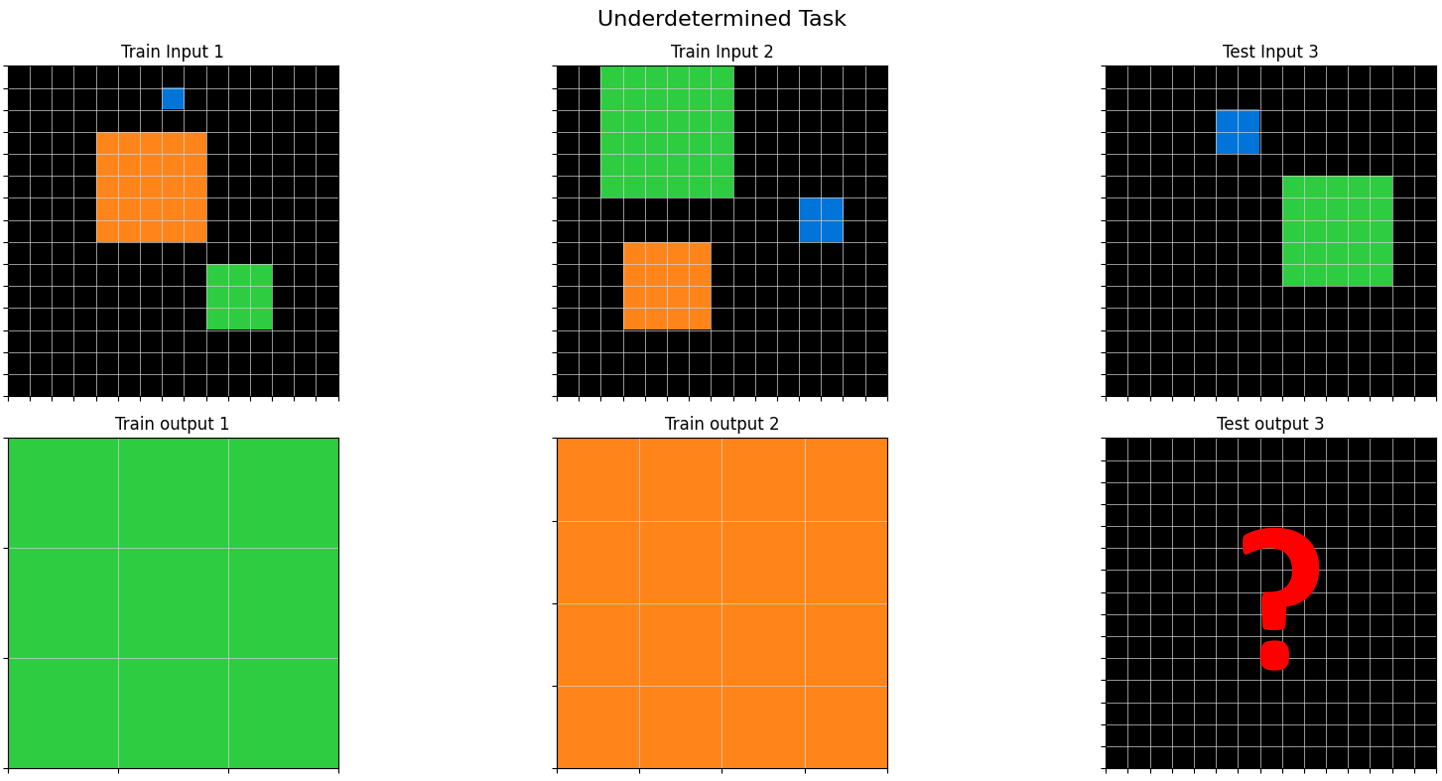
\includegraphics[width=0.6\columnwidth]{Figures/Underdetermined_Task.png}
    \caption{Underdetermined task. While the rule is clear from the two examples: "select the middle-sized object", it is impossible to apply this rule to the test example.}
    \label{fig:Underdetermined Task}
\end{figure}
\end{itemize}

Avoiding over and under-determination of tasks is a very difficult challenge, that has no obvious algorithmic solution since there is no good algorithmic solver. Moreover, it is very difficult to account for all edge cases; for instance, in the underdetermined task in Figure \ref{fig:Underdetermined Task}, we would need to include a specific constraint in our generator that specifies that when generating tasks using the transformation "Select middle sized object", there must always be an odd number of objects. However, it is not the only condition that must be added, we must also ensure that all objects are of distinct sizes, and avoid size ambiguity (e.g. between rows, columns) that would make the task overdetermined. One can see how the problem gets exponentially more challenging when combining different independent transformations for composed tasks. As such, we are aware that our generation paradigm is limited in that it is likely to contain underdetermined and overdetermined tasks. 

\subsubsection{ARC World Model}

Another important challenge is to build a generator that would be as diverse as possible. By diversity, we mean the number of diverse tasks (rules) that our generator is able to produce task examples for. Building a generator with large diversity is challenging for two main reasons: 1) it is incredibly time-consuming to list all the possible concepts that a generator could have access to, and 2) the more concepts we include, the less obvious it is to combine them with one another, as explained previously. Diversity is also difficult to measure, it would be impossible to quantify this for humans, as they understand all the concepts given to them, they freely can assess whether two given concepts are compatible and build a task in a format that would make the rule hold, thus neither being over nor underdetermined.

This significantly hinders our capacity to reach a dataset which is a good basis for a "ARC World Model", as it is not diverse enough in its generation process to provide this basis. Furthermore, the limitation in diversity also limits our capacity to study sample efficiency, which often needs a lot more variety - especially in meta learning frameworks. 

\subsubsection{Future Avenues}

To make progress in ARC, we believe that our generator is a good contribution, but that it is best combined with the other generators presented in the Related Works section, which all provide different advantages and properties. The researcher motivated in building an "ARC World Model" should indeed particularly be interested in combining different datasets, as they all contain peculiarities and biases that are unique to the generator. Building a general world model must therefore be pursued through the combination of these different datasets. 

Regarding the objectives of enabling study of generalization, sample efficiency and compositionality, as well as research avenues relevant for ARC such as symbolic parsing and overcoming the knowledge acquisition bottleneck \cite{symbolicAISOTA}, we believe that our generator brings a sufficient contribution for systematic research. 